% Intended LaTeX compiler: xelatex
\documentclass[10pt, svgnames]{beamer}
\usepackage{graphicx}
\usepackage{longtable}
\usepackage{wrapfig}
\usepackage{rotating}
\usepackage[normalem]{ulem}
\usepackage{amsmath}
\usepackage{amssymb}
\usepackage{capt-of}
\usepackage{hyperref}
\usetheme{metropolis}
\author{Sappinandana Akamphon}
\date{}
\title{Power Screws}
\usepackage{booktabs}
\institute{Department of Mechanical Engineering, TSE}
\usepackage{amsmath}
\usepackage[mathrm=sym]{unicode-math}
\setmathfont{FiraMath-Light}
\AtBeginSection[]{\begin{frame}{Outline}\tableofcontents[currentsection]\end{frame}}
\hypersetup{
 pdfauthor={Sappinandana Akamphon},
 pdftitle={Power Screws},
 pdfkeywords={},
 pdfsubject={},
 pdfcreator={Emacs 30.0.50 (Org mode 9.6)}, 
 pdflang={English}}
\begin{document}

\maketitle

\section{Overview of Power Screws}
\label{sec:org6825514}

\begin{frame}[label={sec:org43b97c1}]{What is a Power Screw?}
\begin{columns}
\begin{column}{0.5\columnwidth}
\begin{center}
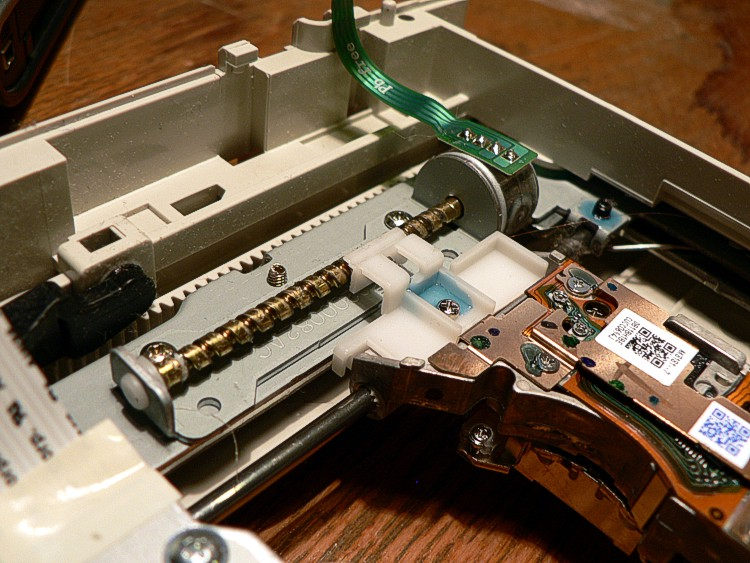
\includegraphics[width=.9\linewidth]{pictures/dvd-drive-screw.jpg}
\end{center}
\end{column}

\begin{column}{0.5\columnwidth}
\begin{itemize}
\item Accurate screw used to push a nut with load along the screw

\item Nut is kept from rotating, so it moves along the screw

\item Transform rotation (torque) into linear motion (axial force)

\item Similar to screw fasteners, but used for motion rather than clamping
\end{itemize}
\end{column}
\end{columns}
\end{frame}

\begin{frame}[label={sec:orgb7b33fe}]{What is a Power Screw Used for?}
\begin{center}
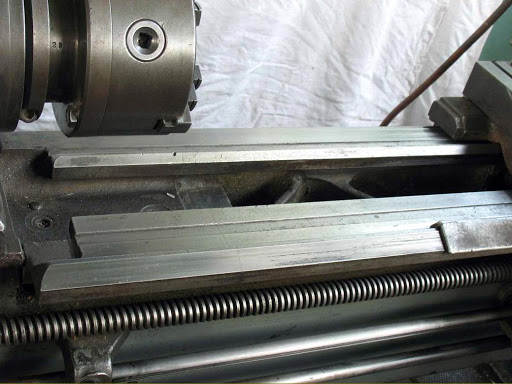
\includegraphics[width=.9\linewidth]{pictures/screw-in-lathe.jpg}
\end{center}
\end{frame}

\section{Types of Power Screws}
\label{sec:org7943fbc}

\begin{frame}[label={sec:orga65dcff}]{Lead Screws vs Ball Screws}
\begin{columns}
\begin{column}{0.5\columnwidth}
\begin{figure}[htbp]
\centering
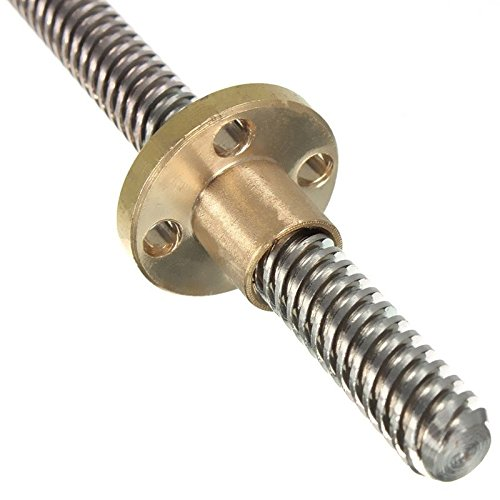
\includegraphics[width=.9\linewidth]{pictures/lead-screw-closeup.jpg}
\caption{Lead Screw}
\end{figure}
\end{column}

\begin{column}{0.5\columnwidth}
\begin{figure}[htbp]
\centering
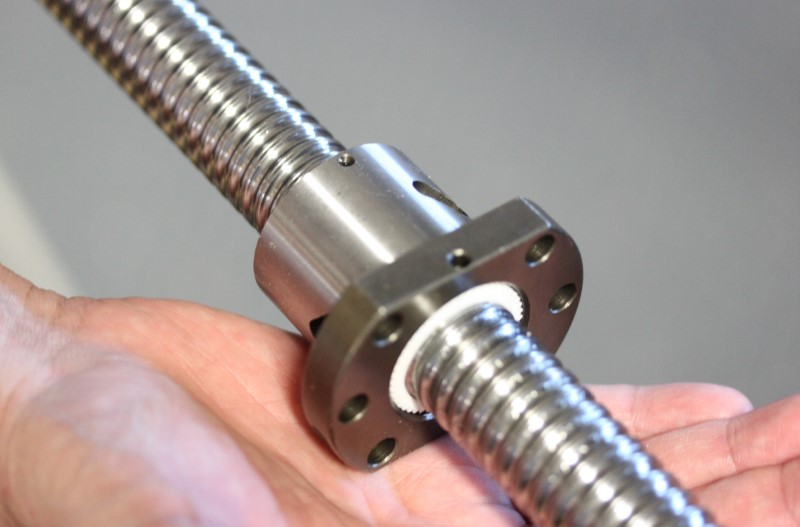
\includegraphics[width=.9\linewidth]{pictures/ball-screw-closeup.JPG}
\caption{Ball Screw}
\end{figure}
\end{column}
\end{columns}
\end{frame}

\begin{frame}[label={sec:orgca56c29}]{Lead Screws}
\begin{center}
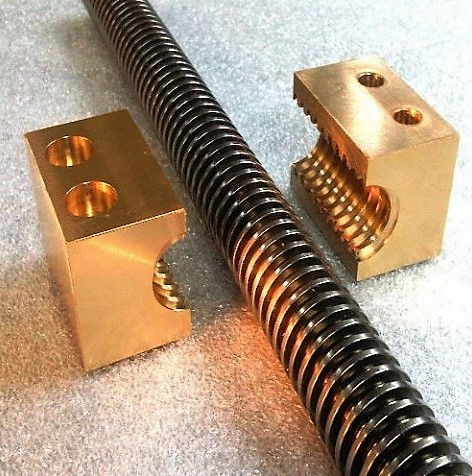
\includegraphics[height=0.9\textheight]{./pictures/lead-screw.jpg}
\end{center}
\end{frame}

\begin{frame}[label={sec:org2ac5614}]{Lead Screw Geometry}
\begin{center}
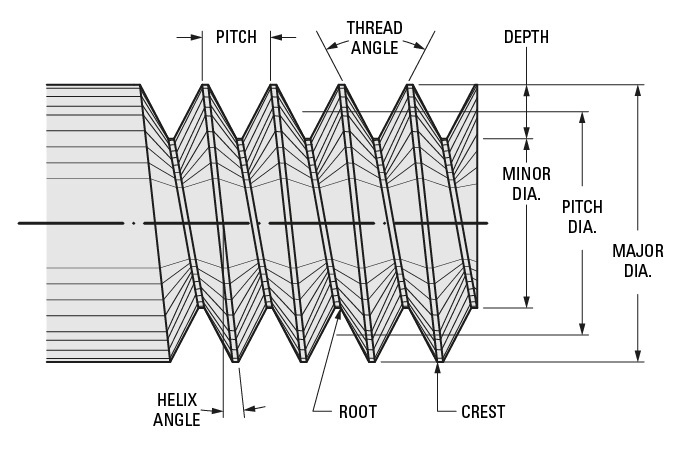
\includegraphics[width=.9\linewidth]{pictures/screw-thread.jpg}
\end{center}
\end{frame}

\begin{frame}[label={sec:orgaa837a8}]{Ball Screws}
\begin{itemize}
\item Bearing + Lead screw = Ball screw

\item Ball screws: recirculating ball bearing, expensive, up to 95\%
efficiency

\begin{center}
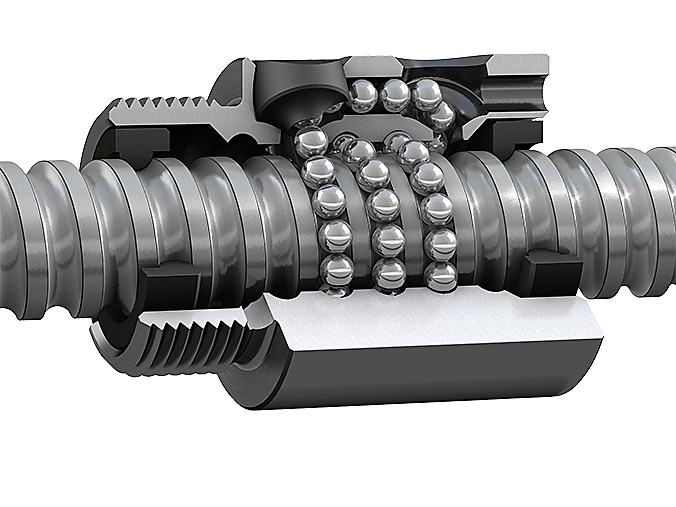
\includegraphics[width=.9\linewidth]{pictures/ball-screw.png}
\end{center}
\end{itemize}
\end{frame}

\begin{frame}[label={sec:org60e9012}]{Ball Screw Geometry}
\begin{center}
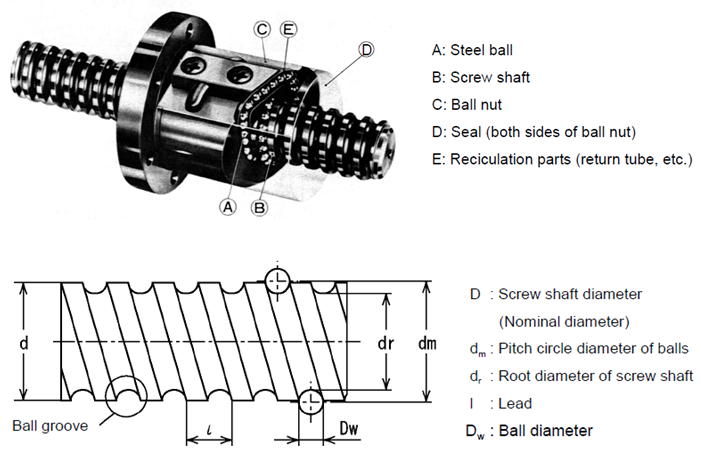
\includegraphics[width=.9\linewidth]{pictures/ball-screw-geometry.png}
\end{center}
\end{frame}

\begin{frame}[label={sec:orgc8e101b}]{Thread Profiles}
\begin{center}
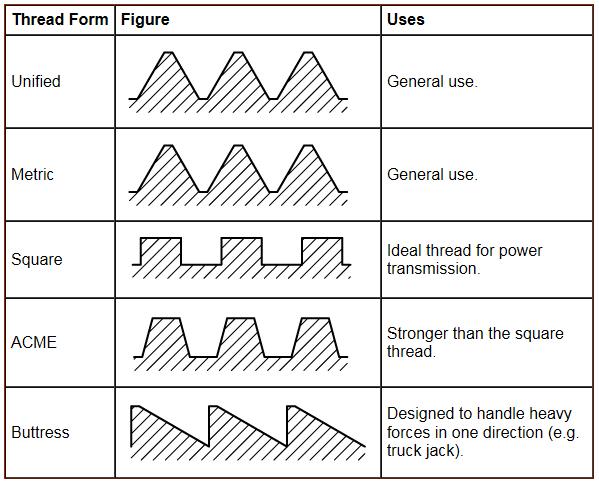
\includegraphics[width=.9\linewidth]{./pictures/thread-types.png}
\end{center}
\end{frame}

\begin{frame}[label={sec:org676ad4d}]{Lead vs Ball Screws}
\begin{center}
\begin{tabular}{ll}
\toprule
Lead & Ball\\\empty
\midrule
Inexpensive + Less complex & More efficient\\\empty
Self-locking & Lower temperature\\\empty
More quiet & Lubrication required\\\empty
\bottomrule
\end{tabular}
\end{center}
\end{frame}

\section{Installation}
\label{sec:org8062269}

\begin{frame}[label={sec:org30c7e97}]{Mounting}
\begin{center}
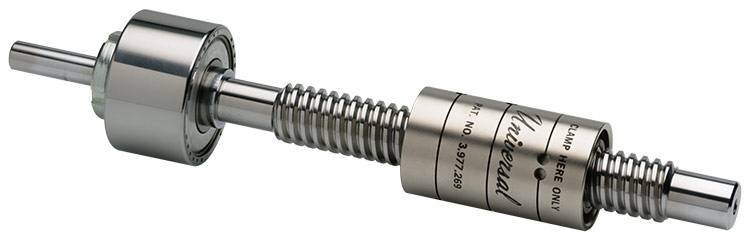
\includegraphics[width=.9\linewidth]{./pictures/thrust-bearing.jpg}
\end{center}

\begin{columns}
\begin{column}{0.5\columnwidth}
\begin{center}
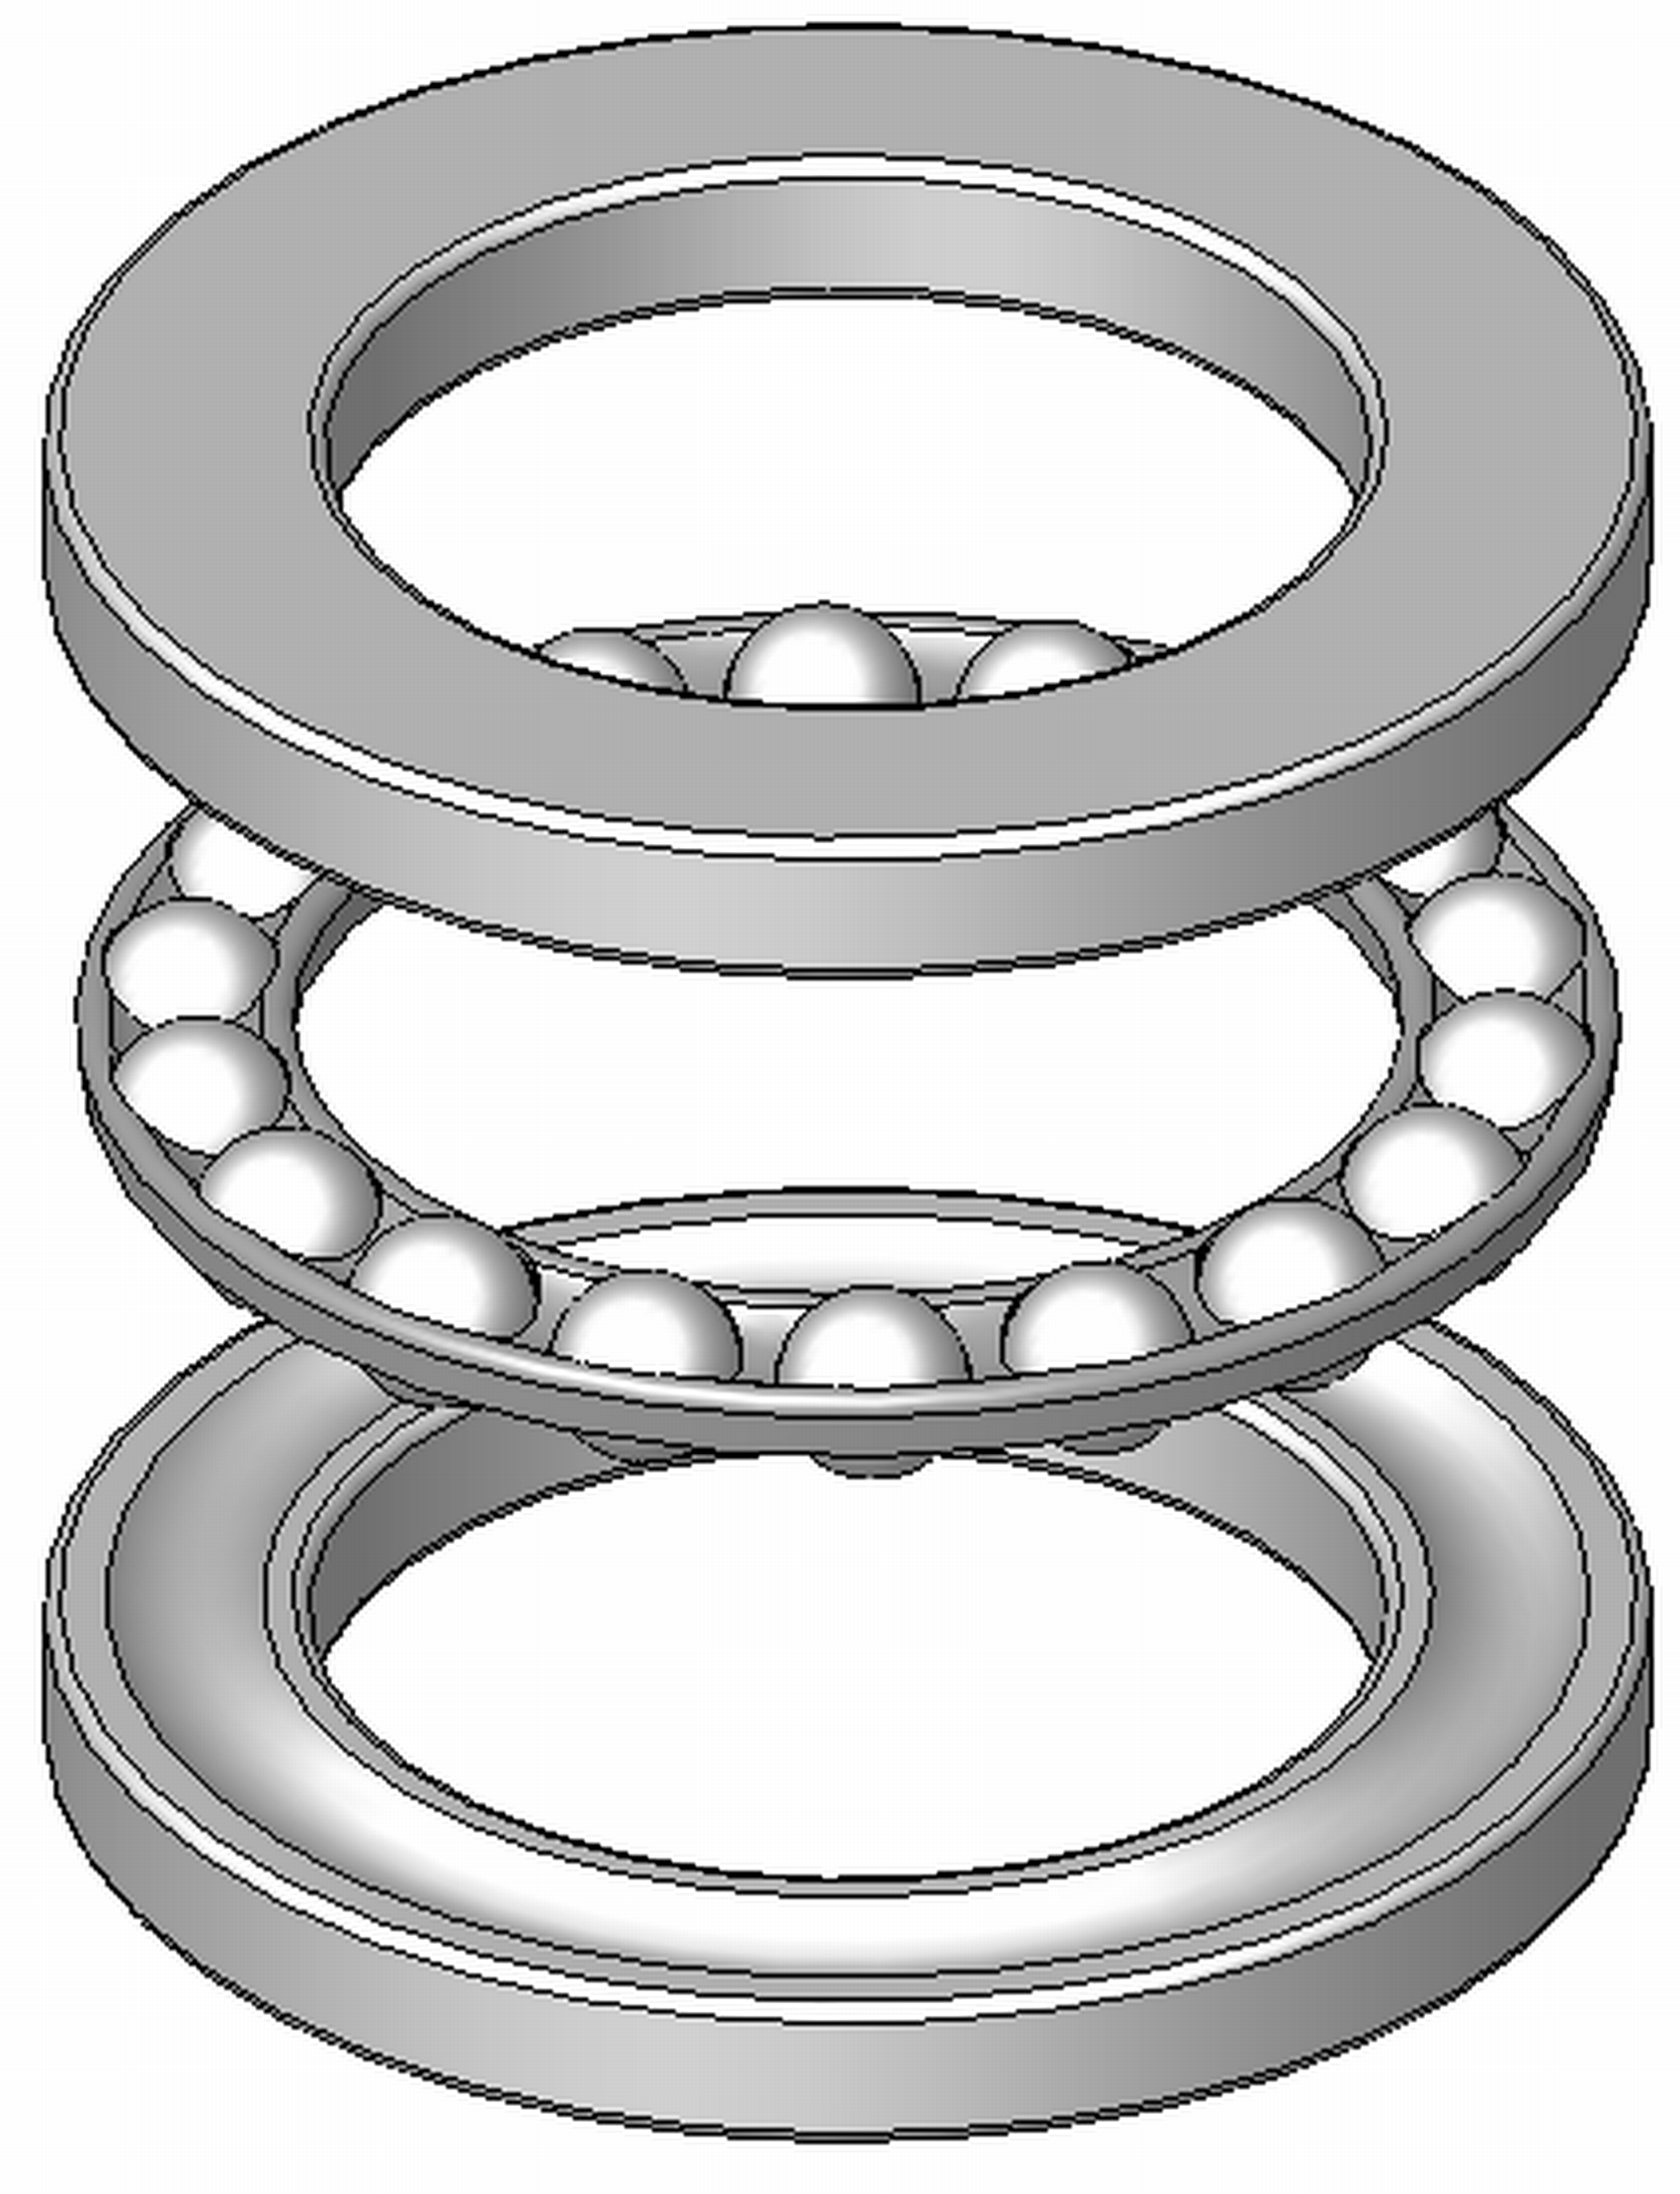
\includegraphics[height=0.5\textheight]{./pictures/thrust-bearing-detailed.png}
\end{center}
\end{column}

\begin{column}{0.5\columnwidth}
\begin{itemize}
\item Power screws should be mounted with bearings that can take thrust (axial) loads
\end{itemize}
\end{column}
\end{columns}
\end{frame}

\begin{frame}[label={sec:orgaad56d3}]{Mounting II}
\begin{itemize}
\item For heavy loads, linear bearings may be needed
\end{itemize}

\begin{center}
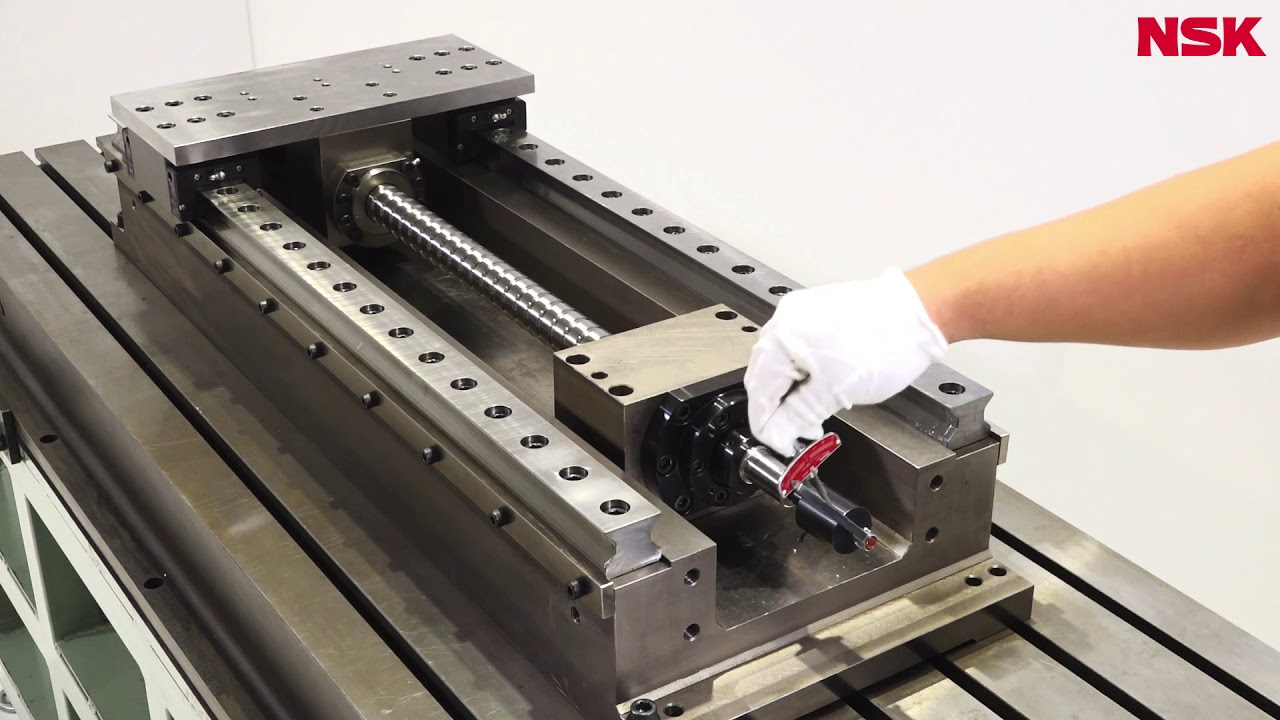
\includegraphics[width=.9\linewidth]{./pictures/screw-mounting.jpg}
\end{center}
\end{frame}

\section{Power Screws Analysis}
\label{sec:org4d2c496}

\begin{frame}[label={sec:org3f9bc70}]{Forces on Power Screws}
\begin{columns}
\begin{column}{0.6\columnwidth}
\begin{center}
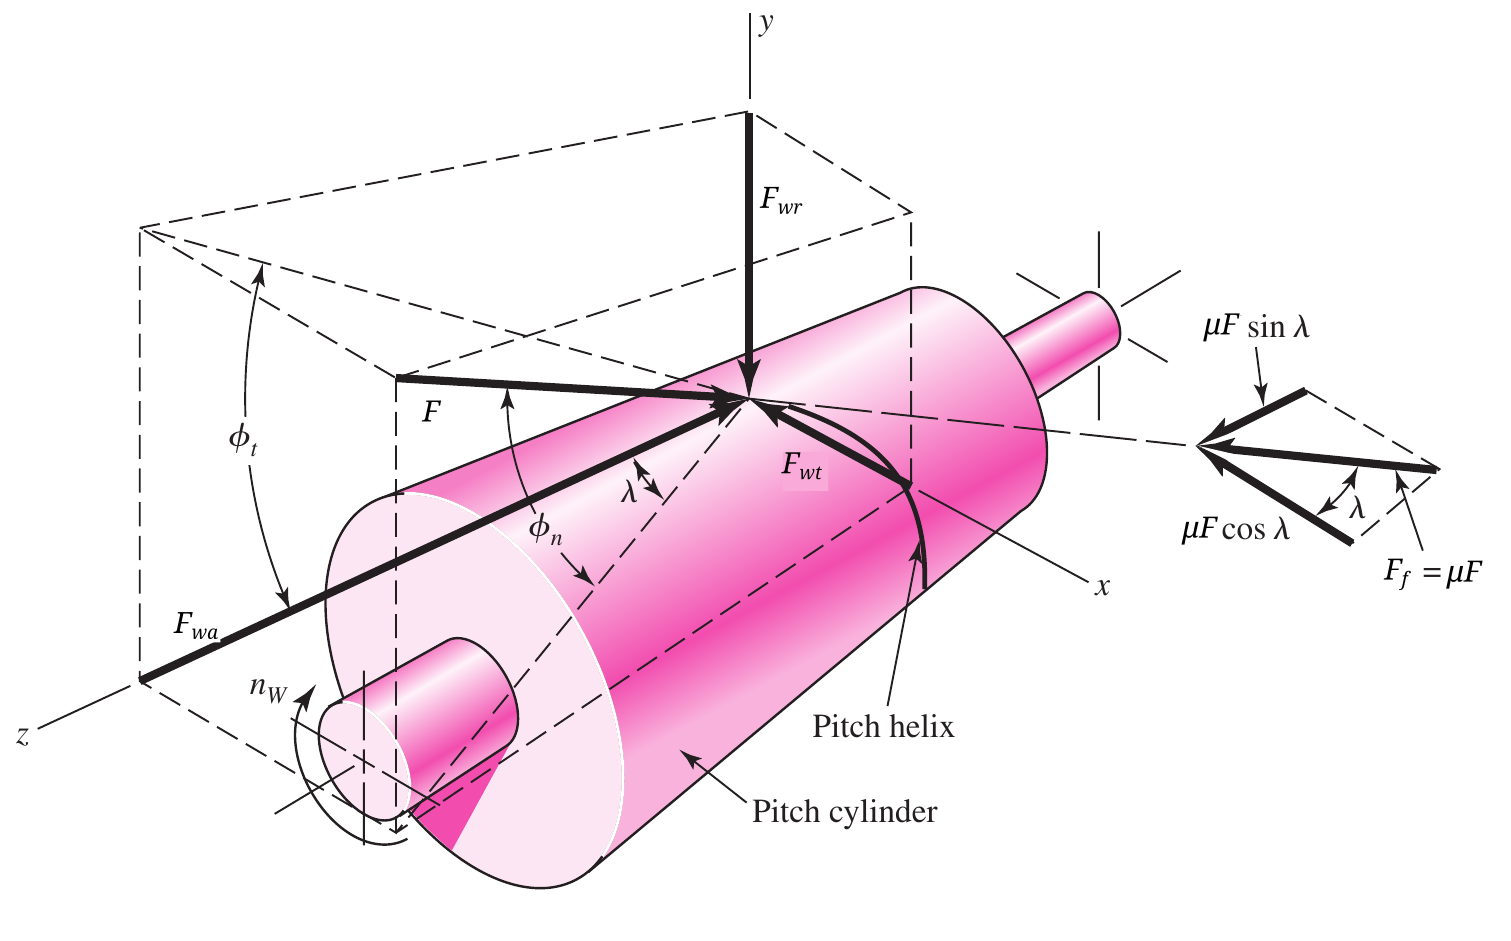
\includegraphics[width=\textwidth]{./pictures/screw-forces.jpg}
\end{center}

\begin{figure}
  \begin{tikzpicture}[>=latex]
    \draw [->, ultra thick] (0,0) --++ (0:3) node(right){} node[midway, below]{$\pi d$};
    \draw [->, ultra thick] (right.center) --++ (90:2) node(top){} node[midway, right]{$l$};
    \draw [->, dashed] (0,0) -- (top.center);
    \node [xshift=0.7cm, yshift=0.2cm]{$\lambda$};
  \end{tikzpicture}
\end{figure}
\normalcolor
\end{column}

\begin{column}{0.5\columnwidth}
\begin{align*}
  F_{t} &= F \cos \phi_{n} \sin \lambda + \mu F \cos \lambda \\
  F_{r} &= F \sin \phi_{n} \\
  F_{a} &= F \cos \phi_{n} \cos \lambda - \mu F \sin \lambda
\end{align*}

\begin{align*}
  % x = \frac{p \theta}{2\pi} \\
  \tan \lambda = \frac{v_{nut}}{v_{shaft}} = \frac{l}{\pi d}
\end{align*}

\begin{description}
\item[{\(\lambda\)}] lead angle
\item[{\(l\)}] screw lead (pitch)
\item[{\(d\)}] screw diameter
\end{description}
\end{column}
\end{columns}
\end{frame}

\begin{frame}[label={sec:org0f19ab8}]{Power Screw Efficiency}
\begin{itemize}
\item Input and output power

\begin{align*}
  H_{in} &= F_{t} v_{shaft} = T_{shaft}\omega_{shaft} \\
  H_{out} &= F_{a} v_{nut}
\end{align*}

\begin{align*}
  \eta &= \frac{F_{a}v_{nut}}{F_{t}v_{shaft}} = \frac{F_{nut}v_{nut}}{T_{shaft}\omega_{shaft}} \\
  \eta_{raise} &= \frac{\cos \phi_{n} \cos \lambda - \mu \sin \lambda}{\cos \phi_{n} \sin \lambda + \mu \cos \lambda} \tan \lambda \\
       &= \frac{\cos \phi_{n} - \mu \tan \lambda}{\cos \phi_{n} + \mu \cot \lambda} \\
  \eta_{lower} &= \frac{\cos \phi_{n} + \mu \tan \lambda}{\cos \phi_{n} - \mu \cot \lambda}
\end{align*}
\end{itemize}
\end{frame}

\begin{frame}[label={sec:orgc786e65}]{Required Torque}
\begin{align*}
  T_{raise} &= \frac{F_{nut}v_{nut}}{\omega_{shaft}} \frac{\cos \phi_{n} + \mu \cot \lambda}{\cos \phi_{n} - \mu \tan \lambda} \\
            &= \frac{F_{nut}v_{nut}}{v_{shaft}/(d/2)} \frac{\cos \phi_{n} + \mu \cot \lambda}{\cos \phi_{n} - \mu \tan \lambda} \\
            &= \frac{F_{nut}d \tan \lambda}{2} \frac{\cos \phi_{n} + \mu \cot \lambda}{\cos \phi_{n} - \mu \tan \lambda} \\
  T_{lower} &= \frac{F_{nut}d \tan \lambda}{2} \frac{\cos \phi_{n} - \mu \cot \lambda}{\cos \phi_{n} + \mu \tan \lambda} \\
\end{align*}

\begin{itemize}
\item set \(F_{nut} = F\) to determine required torque
\end{itemize}
\end{frame}

\begin{frame}[label={sec:orga477ea1}]{Required Torque II}
\begin{itemize}
\item Power screw sizes are usually given in lead \(l\), (major) diameter, effective (median) diameter \(d\), root (minor) diameter
\end{itemize}

\begin{align*}
  \tan \lambda &= \frac{l}{\pi d} \\
  T_{raise} &= \frac{F_{nut}d \tan \lambda}{2} \frac{\cos \phi_{n} + \mu \cot \lambda}{\cos \phi_{n} - \mu \tan \lambda} \\
           &= \frac{F_{nut}d}{2} \frac{l}{\pi d} \frac{\cos \phi_{n} + \mu \frac{\pi d}{l}}{\cos \phi_{n} - \mu \frac{l}{\pi d}} \\
           &= \frac{F_{nut}d}{2} \frac{l \cos \phi_{n} + \mu \pi d}{\pi d \cos \phi_{n} - \mu l} \\
  T_{lower} &= \frac{F_{nut}d}{2} \frac{l \cos \phi_{n} - \mu \pi d}{\pi d \cos \phi_{n} + \mu l} \\
\end{align*}
\end{frame}

\begin{frame}[label={sec:org8ee0539}]{Self-Locking}
\begin{itemize}
\item Similar to worm gears
\end{itemize}

\begin{align*}
  F_{t} &= F \cos \phi_{n} \sin \lambda - \mu F \cos \lambda \leqslant 0 \\
  \mu &\geqslant \cos \phi_{n} \tan \lambda
\end{align*}

\begin{itemize}
\item Possible in lead screws (\(\mu\) > 0), \alert{NOT} in ball screws (\(\mu\) \(\approx\) 0).
\item This makes lead screws desirable in vertical application: self-locking prevents weight drop
\end{itemize}
\end{frame}

\begin{frame}[label={sec:org4f32d08}]{Buckling}
\begin{itemize}
\item Buckling is a common failure in shafts

\item Put shafts in TENSION whenever possible

\item Power screws can easily generate forces that will buckle them

\item Heavy loads should be PULLED, not PUSHED
\end{itemize}
\end{frame}

\begin{frame}[label={sec:org6536e25}]{Shaft Whirling}
\begin{itemize}
\item Shafts (or screws) that spins too fast can excite shaft bending
(whirling or whip) \(\rightarrow\) bearing failure

\begin{align*}
  \omega_{\max} \leqslant 0.8\omega_{1}
\end{align*}
\end{itemize}
\end{frame}

\begin{frame}[label={sec:orga862666}]{Buckling and Whirling Formula}
\begin{align*}
  \omega_{1} &= k^{2} \sqrt{ \frac{EI}{A\rho L^{4}} } \\
  P_{cr} &= \frac{cEI}{L^{4}}
\end{align*}

\begin{center}
\begin{tabular}{lrr}
\toprule
End conditions & \(k\) & \(c\)\\\empty
\midrule
cantilevered & 1.88 & 2.47\\\empty
simply supported & 3.14 & 9.87\\\empty
fixed-simple & 3.93 & 20.2\\\empty
fixed-fixed & 4.73 & 39.5\\\empty
\bottomrule
\end{tabular}
\end{center}
\end{frame}

\begin{frame}[label={sec:orgb122774}]{Example: Power Screw Design}
We need to drive a 50-kg mass vertically. The selected lead screw has \(\mu\) = 0.1, \(\phi_n\) = 0\(^{\circ}\), \(l\) = 2 mm, \(d\) = 10 mm, \(E\) = 210 GPa. Determine the required torque to drive this mass
\end{frame}

\begin{frame}[label={sec:org065e31a}]{Solution}
Required torque is (typically) \(T_{raise}\), as it is usually larger.

\begin{align*}
  T_{raise} &= \frac{F_{nut}d}{2} \frac{l \cos \phi_{n} + \mu \pi d}{\pi d \cos \phi_{n} - \mu l} \\
            &= \frac{500(0.01)}{2} \frac{0.002(1) + 0.1 \pi (0.01)}{\pi (0.01)(1) - 0.1(0.002)} \\
            &= 0.412 \text{ N-m}
\end{align*}
\end{frame}
\end{document}